\chapter{Defining research questions and study setting}
\label{ch:study_setting}

The experiments in the following chapter form the basis for our analysis of the watermarking methods, with which we want to answer the following research questions.

%overall question:
\textbf{How can we define the most fitting watermarking method depending on the ML setting?}

%relevance:
Research on watermarking ML models is growing and so is the number of papers proposing new watermarking methods.
%why non-trivial:
Some of the papers do a comprehensive evaluation of their watermarking method, testing it on different datasets and architectures but rarely compare it to all existing methods. Moreover, usually authors pick the best results for their paper without pointing out the weaknesses of the presented method.
%how to adress this question:
With the independent implementation and evaluation in this thesis, we want to find potential influences of a ML setting on the \textbf{effectiveness}, \textbf{fidelity} and \textbf{robustness} of a watermarking method.
%how to measure:
We answer this question by designing a study setting, in which we are going to measure the \textbf{effectiveness}, \textbf{fidelity} and \textbf{robustness} by computing the watermark accuracy (for effectiveness) and test accuracy (for fidelity) after embedding the watermark, and computing the watermark accuracy after an attack (for robustness).

We break down this question into three specific subquestions:
%breaking overall question down into...
\begin{enumerate}
\item \textbf{To what extend is a more complex model able to hold more watermark information (a bigger trigger set) without compromising test accuracy?} A more complex model has more parameters and therefore more "space" to hide a watermark. On the other hand, a model with fewer parameters might rather give up on the main classification task in order to overfit on the trigger set. We want to answer this question by performing experiments with various trigger set sizes and architectures and measuring the difference in test accuracy after the watermark embedding.

\item \textbf{To what extend does the trigger set size influence the effectiveness, fidelity and robustness of a watermarking method?} A bigger trigger set size could mean better robustness, since an attacker would need more time or data to, e.g., remove the watermark by fine-tuning. On the other hand, a bigger trigger set could also result in worse fidelity. For effectiveness, a smaller trigger set size, could mean that the model does not learn the watermark at all, as the ratio compared to the original dataset is too low and it prioritises on the original dataset. These are hypotheses that we want to follow under this research question.

\item \textbf{To what extend does the complexity of the model influence the effectiveness, fidelity and robustness of the watermarking method?} Similar to the question above, we assume that the complexity of a model plays a role on the effectiveness, fidelity and robustness of a watermarking method. With our experiments, we want to find out if our assumption is true.
\end{enumerate}

%for the RQs: I usually recommend to define research questions in a hierarchical form, starting from an overall questions defining the scope of the problem to be addressed, and subsequently breaking this down into 3-4 atual and precise research questions (RQ) which can, in turn, be broken down into further subquestions if necessary.
%Each individual research question should consist of

%the question, preferably phrased quantitatievely (to what extent)
%1-2 sentences why it is a relevant / interesting question
%1-2 sentences wy it is a non-trivial question (i.e. not simply solved by state of the art knowledge)
%1-2 sentences how to address this question methodologically (which theoretical concepts, analyses, experiments, measurements)
%1-2 sentences on how to measure the degree of answering / solving the research challenge, preferably quantitativle in an objective manner, if necessary subjectively including an according study design.

We choose our subset of watermarking methods according to the following criteria. The chosen watermarking method must
\begin{itemize}
    \item be a black-box and backdoor-based watermarking method, as these are more practical than white-box methods.
    \item focus on trigger set generation rather than trigger labelling, as trigger images are the first step to analyse and optimise. An analysis of watermarking methods regarding trigger labelling are kept for future work.
    \item be a watermarking method that does not build upon another watermarking method, as in a first step we want to identify the aspects which make the basic methods perform better.
\end{itemize}

\begin{table}
\small
\renewcommand{\arraystretch}{1.1}
\centering

\begin{threeparttable}
\caption{Study settings in selected papers.}
\label{tab:models-and-datasets}
%\rowcolors{2}{white}{gray!15}
\begin{tabular}{|l|l|l|l|}
\hline
\textbf{Method}               & \textbf{Type}                & \textbf{Dataset}                                                                             & \textbf{Architecture}                                                                                                                                                                                                   \\ \hline
%\textit{Blackmarks} \cite{chen_blackmarks_2019}           & perturbation               & \begin{tabular}[c]{@{}l@{}}MNIST,\\ CIFAR-10\end{tabular}                           & \begin{tabular}[c]{@{}l@{}}WRN \cite{zagoruyko_wide_2017},\\ AlexNet \cite{krizhevsky_imagenet_2017},\\ custom DNN\end{tabular}                                                                                                                                           \\ \hline
%EvolutionaryGen      & pattern, (noise)    & \begin{tabular}[c]{@{}l@{}}MNIST,\\ CIFAR-10\end{tabular}                           & \begin{tabular}[c]{@{}l@{}}ResNet-18,\\ ResNet-50,\\ DenseNet-121,\\ VGG-16\end{tabular}                                                                                                                       \\ \hline
\textit{ExponentialWeighting} \cite{namba_robust_2019} & in-distribution     & \begin{tabular}[c]{@{}l@{}}MNIST,\\ CIFAR-10,\\ CIFAR-100,\\ GTSRB\end{tabular}     & ResNet32                                                                                                                                                                                                       \\ \hline
\textit{FrontierStitching} \cite{merrer_adversarial_2019}    & perturbation        & MNIST                                                                               & \begin{tabular}[c]{@{}l@{}} MLP \tnote{1} \; ,\\ CNN \tnote{2} \; ,\\ IRNN \tnote{3} \;  \end{tabular}                                                                                                                                \\ \hline
%HowToProve           & noise/pattern       & \begin{tabular}[c]{@{}l@{}}MNIST,\\ CIFAR-10\end{tabular}                           & \begin{tabular}[c]{@{}l@{}}LeNet-1/2/5,\\ VGG-11/13/16/19,\\ ResNet-18/34/101,\\ PreActResNet-34,\\ GoogleNet,\\ DPN-26,\\ MobileNetV2\end{tabular} \\ \hline
\textit{PiracyResistant} \cite{li_piracy_2020}     & pattern             & \begin{tabular}[c]{@{}l@{}}MNIST,\\ CIFAR-10,\\ GTSRB,\\ Youtube Faces\end{tabular} & custom DNN                                                                                                                                                                                                     \\ \hline
\textit{ProtectingIP} \cite{zhang_protecting_2018}        & pattern, noise, OOD & \begin{tabular}[c]{@{}l@{}}MNIST,\\ CIFAR-10\end{tabular}                           & custom DNN                                                                                                                                                                                                     \\ \hline
\textit{WeaknessIntoStrength} \cite{adi_turning_2018} & OOD                 & \begin{tabular}[c]{@{}l@{}}CIFAR-10,\\ CIFAR-100,\\ ImageNet\end{tabular}           & ResNet-18                                                                                                                                                                                                      \\ \hline
\textit{WMEmbeddedSystems} \cite{guo_evolutionary_2019}    & pattern             & \begin{tabular}[c]{@{}l@{}}MNIST,\\ CIFAR-10\end{tabular}                           & \begin{tabular}[c]{@{}l@{}}LeNet-5,\\ VGG-16,\\ ResNet50,\\ DenseNet-121\end{tabular}                                                                                                                            \\ \hline
\end{tabular}

\medskip % some vertical separation
\begin{tablenotes}
\footnotesize  % nothing is optional in 'tablenotes'
\item[1] \url{https://keras.rstudio.com/articles/examples/mnist_mlp.html}
\item[2] \url{https://keras.rstudio.com/articles/examples/mnist_cnn.html}
\item[3] \url{https://keras.rstudio.com/articles/examples/mnist_irnn.html}

\end{tablenotes}
\end{threeparttable}
\end{table}


Following these criteria, we decided on the watermarking methods that are listed in \cref{tab:models-and-datasets}. This table includes also the experimental setup in the corresponding papers. Our choice of the datasets and architectures is very much inspired by the choice in the papers.

%I think it would be very important to also compare your work to chen\_performance\_2018 in more detail - what are the difference in the studies? you have more frameworks, of course, but are there also other differences in what you measure, how you measure, ... ?

A work by Chen et al. \cite{chen_performance_2018} compares $5$ watermarking methods \cite{uchida_embedding_2017,rouhani_deepsigns_2019, zhang_protecting_2018, adi_turning_2018, merrer_adversarial_2019}, both white-box and black-box watermarking methods. It is worth noting that this is not an independent comparison, since the authors are also the authors of one of the considered watermarking methods, DeepSigns \cite{rouhani_deepsigns_2019}, and it performs best in most of the results. DeepSigns can be implemented as both white-box and black-box (cf. \cref{ch:sota}) and therefore they are comparing it to one white-box and three black-box methods. Even though the method \textit{can} be considered as black-box, it is not backdoor-based and relies on the prediction vector for watermark verification, which might not be available in all settings. They implement the methods and train the black-box watermarked models with a trigger set size of $20$ on four different architectures, and the white-box watermarked models on three different architectures. Both watermarking types are trained on MNIST and CIFAR-10, the black-box type also on ImageNet. They evaluate the models regarding fidelity, robustness against fine-tuning, parameter pruning and watermark overwriting, and integrity, i.e. the watermarking method should have a minimal false positive rate. Although the comparison lacks on different settings and independence, the evaluation of fidelity and robustness is done in a similar fashion to ours. However, they do not present results on effectiveness, i.e. the watermark accuracy of the watermarked model.

%from SotA:
%As the first work in this field, an empirical study by Chen et al. \cite{chen_performance_2018} investigates five model watermarking schemes (two white-box \cite{uchida_embedding_2017, rouhani_deepsigns_2019}, and four black-box \cite{merrer_adversarial_2019, adi_turning_2018, zhang_protecting_2018}), and performs an evaluation of fidelity of the models, as well as estimating the robustness against three attacks (model fine-tuning, parameter pruning, and watermark overwriting), thus providing an important early comparison of the effectiveness of techniques. 

In order to answer the research questions, we have to evaluate the watermarking methods in a common and independent study setting. There are some parameters that we would like to fix to specific values, and others that we would like to vary in order to draw conclusions. We modify the following parameters, as these are the usual parameters that are modified by the research papers. We, however, vary also the size of trigger set, which is rarely done by other authors.

\begin{itemize}
    \item \textbf{Complexity of architecture}: we choose eight state-of-the-art architectures, inspired by the experimental setup in the proposed papers (cf. \cref{tab:models-and-datasets}), i.e. SimpleNet, LeNet-1/3/5 for MNIST and DenseNet, ResNet-18/34/50 for CIFAR-10.
    \item \textbf{Size of training set and images}: a variation in the size of training set and examples is unfortunately in this stage of the work not possible. We have chosen two datasets which both have a similar size of training set and a similar (small) size of images. 
    \item \textbf{Color depth}: we choose one RGB and one greyscale dataset, i.e. CIFAR-10 and MNIST.
    \item \textbf{Size of trigger set:} we vary between three trigger set sizes, i.e. 0.04\%, 0.2\% and 1\% of the training set.
    \item \textbf{Embedding type}: we use two embedding types. Embedding from scratch -- training the model on the union of the training dataset and the trigger set from the very beginning of training; and embedding on a pre-trained model -- embedding the watermark as a fine-tuning step after training the model only on the original data.
    \item \textbf{Complexity of attacks}: we choose two common attacks, i.e. parameter pruning and fine-tuning, to test the robustness, they both differ in overhead.
\end{itemize}

%compare a total of (3*7 + 4)*7 + (3*6+4)*1 + (2*8)*1 = 213 models

In the following sections, we present the datasets and neural networks that we use for the experiments.

\section{Datasets}
We use four different datasets: two datasets (MNIST and CIFAR-10) for training the models, and another two datasets (EMNIST and CINIC-10) for carrying out the fine-tuning attacks:
\begin{itemize}
    % http://yann.lecun.com/exdb/mnist/
    \item \textbf{MNIST \cite{lecun_gradient-based_1998}:} is a grayscale handwritten digits dataset consisting of 60,000 training examples and 10,000 test examples. All images have been size-normalized and centered in a fixed-size image of $28\times28$ pixels.
    % https://www.cs.toronto.edu/~kriz/cifar.html
    \item \textbf{CIFAR-10 \cite{krizhevsky_learning_2009}:} is a real-world image dataset containing the classes airplane, car, bird, cat, deer, dog, frog, horse, ship, truck. The dataset consists of 50,000 training examples and 10,000 test examples, all in colour (RGB) and sized $32\times32$ pixels.
    % http://ufldl.stanford.edu/housenumbers/
    %\item \textbf{SVHN \cite{netzer_reading_2011}:} is a real-world digit images dataset containing images of house numbers obtained from Google Street View images. The training set contains 73,257 examples and the test set contains 26,032 examples. The images are in color (RGB) and resized to 32x32 pixels. This dataset is used for fine-tuning attacks on models originally trained on MNIST.
    % https://www.nist.gov/itl/products-and-services/emnist-dataset
    \item \textbf{EMNIST \cite{cohen_emnist_2017}:} is another grayscale handwritten digits dataset. It is derived from the NIST Special Database 19 \cite{grother_NIST_1970} and converted to fixed-size images of $28\times28$ pixels. The EMNIST dataset consists of six different splits, namely ByClass, ByMerge, Balanced, Letters, Digits and MNIST. We use the Digits split, which contains of 280,000 example-label pairs. The EMNIST dataset structure matches directly with MNIST, which makes it convenient to use for our experiments. We use this dataset for fine-tuning attacks on models that were originally trained on MNIST.
    % https://cs.stanford.edu/~acoates/stl10/
    %\item \textbf{STL-10 \cite{coates_analysis_2011}:} is another real-world images dataset, inspired by the CIFAR-10 dataset. It consists of 5,000 training images, 8,000 test images and 100,000 unlabelled images. The classes are airplane, bird, car, cat, deer, dog, horse, monkey, ship, truck. All images are in color (RGB) and have a fixed size of 96x96 pixels.  This dataset is used for fine-tuning attacks on models that were originally trained on CIFAR-10.
    % https://paperswithcode.com/dataset/cinic-10
    \item \textbf{CINIC-10 \cite{darlow_cinic-10_2018}:} is another real-world image dataset that extends CIFAR-10 by adding additionally selected images from ImageNet \cite{russakovsky_imagenet_2015}, resized to $32\times32$ pixels to match the ones from CIFAR-10. images. It is $4.5$ times larger than CIFAR-10, but still smaller (and comprising fewer classes) than ImageNet, and thus creates a bridge between these two datasets. As the classes are exactly the same as for CIFAR-10, we can use this dataset for fine-tuning attacks on models that were originally trained on CIFAR-10.
\end{itemize}

The properties of the datasets are summarised in \cref{tab:datasets} and examples of images from each class are shown in \cref{fig:datasets}. The datasets that we choose for fine-tuning originally consist of more data samples than MNIST and CIFAR-10. However, we use only a subset of these datasets, since fine-tuning is usually performed using a smaller dataset than the original one. In our experiments, we downsample EMNIST and CINIC-10 to the size of MNIST and CIFAR-10, respectively.

\begin{table}
\small
    \centering
    %\rowcolors{2}{white}{gray!15}
    \begin{tabular}{|l|l|l|r|r|}
        \hline
        \textbf{Dataset} & \textbf{Size} & \textbf{Color} & \textbf{Training set} & \textbf{Test set} \\
        \hline
        MNIST & $28\times28$ & grayscale & 60,000 & 10,000 \\
        %\hline
        %SVHN & $32\times32$ & RGB & 73,257 & 26,032 \\
        \hline
        EMNIST Digits & $28\times28$ & grayscale & 240,000 & 40,000 \\
        \hline
        CIFAR-10 & $32\times32$ & RGB & 50,000 & 10,000 \\
        %\hline
        %STL-10 & $96\times96$ & RGB & 5,000 & 8,000 \\
        \hline
        CINIC-10 & $32\times32$ & RGB & 90,000 & 90,000 \\
        \hline
    \end{tabular}
    \caption{Characteristics of the datasets used in the evaluation}
    \label{tab:datasets}
\end{table}
\begin{figure}[t]
    \centering
    
\includegraphics[width = 0.09 \textwidth]{images/datasets/mnist_0.png}
    
\includegraphics[width = 0.09 \textwidth]{images/datasets/mnist_1.png}
    
\includegraphics[width = 0.09 \textwidth]{images/datasets/mnist_2.png}
    
\includegraphics[width = 0.09 \textwidth]{images/datasets/mnist_3.png}
    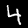
\includegraphics[width = 0.09 \textwidth]{images/datasets/mnist_4.png}
    
\includegraphics[width = 0.09 \textwidth]{images/datasets/mnist_5.png}
    
\includegraphics[width = 0.09 \textwidth]{images/datasets/mnist_6.png}
    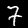
\includegraphics[width = 0.09 \textwidth]{images/datasets/mnist_7.png}
    
\includegraphics[width = 0.09 \textwidth]{images/datasets/mnist_8.png}
    
\includegraphics[width = 0.09 \textwidth]{images/datasets/mnist_9.png}
    
\includegraphics[width = 0.09 \textwidth]{images/datasets/cifar10_0.png}
    
\includegraphics[width = 0.09 \textwidth]{images/datasets/cifar10_1.png}
    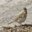
\includegraphics[width = 0.09 \textwidth]{images/datasets/cifar10_2.png}
    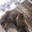
\includegraphics[width = 0.09 \textwidth]{images/datasets/cifar10_3.png}
    
\includegraphics[width = 0.09 \textwidth]{images/datasets/cifar10_4.png}
    
\includegraphics[width = 0.09 \textwidth]{images/datasets/cifar10_5.png}
    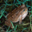
\includegraphics[width = 0.09 \textwidth]{images/datasets/cifar10_6.png}
    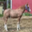
\includegraphics[width = 0.09 \textwidth]{images/datasets/cifar10_7.png}
    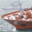
\includegraphics[width = 0.09 \textwidth]{images/datasets/cifar10_8.png}
    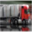
\includegraphics[width = 0.09 \textwidth]{images/datasets/cifar10_9.png}
   % 
\includegraphics[width = 0.09 \textwidth]{images/datasets/svhn_0.png}
    %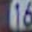
\includegraphics[width = 0.09 \textwidth]{images/datasets/svhn_1.png}
    %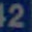
\includegraphics[width = 0.09 \textwidth]{images/datasets/svhn_2.png}
    %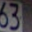
\includegraphics[width = 0.09 \textwidth]{images/datasets/svhn_3.png}
    %
\includegraphics[width = 0.09 \textwidth]{images/datasets/svhn_4.png}
    %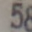
\includegraphics[width = 0.09 \textwidth]{images/datasets/svhn_5.png}
    %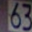
\includegraphics[width = 0.09 \textwidth]{images/datasets/svhn_6.png}
    %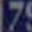
\includegraphics[width = 0.09 \textwidth]{images/datasets/svhn_7.png}
    %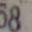
\includegraphics[width = 0.09 \textwidth]{images/datasets/svhn_8.png}
    %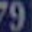
\includegraphics[width = 0.09 \textwidth]{images/datasets/svhn_9.png}
    
\includegraphics[width = 0.09 \textwidth]{images/datasets/emnist_0.jpg}
    
\includegraphics[width = 0.09 \textwidth]{images/datasets/emnist_1.jpg}
    
\includegraphics[width = 0.09 \textwidth]{images/datasets/emnist_2.jpg}
    
\includegraphics[width = 0.09 \textwidth]{images/datasets/emnist_3.jpg}
    
\includegraphics[width = 0.09 \textwidth]{images/datasets/emnist_4.jpg}
    
\includegraphics[width = 0.09 \textwidth]{images/datasets/emnist_5.jpg}
    
\includegraphics[width = 0.09 \textwidth]{images/datasets/emnist_6.jpg}
    
\includegraphics[width = 0.09 \textwidth]{images/datasets/emnist_7.jpg}
    
\includegraphics[width = 0.09 \textwidth]{images/datasets/emnist_8.jpg}
    
\includegraphics[width = 0.09 \textwidth]{images/datasets/emnist_9.jpg}
    %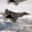
\includegraphics[width = 0.09 \textwidth]{images/datasets/stl10_0.png}
    %
\includegraphics[width = 0.09 \textwidth]{images/datasets/stl10_1.png}
    %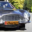
\includegraphics[width = 0.09 \textwidth]{images/datasets/stl10_2.png}
    %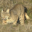
\includegraphics[width = 0.09 \textwidth]{images/datasets/stl10_3.png}
    %
\includegraphics[width = 0.09 \textwidth]{images/datasets/stl10_4.png}
    %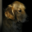
\includegraphics[width = 0.09 \textwidth]{images/datasets/stl10_5.png}
    %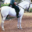
\includegraphics[width = 0.09 \textwidth]{images/datasets/stl10_6.png}
    %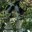
\includegraphics[width = 0.09 \textwidth]{images/datasets/stl10_7.png}
    %
\includegraphics[width = 0.09 \textwidth]{images/datasets/stl10_8.png}
    %
\includegraphics[width = 0.09 \textwidth]{images/datasets/stl10_9.png}
    \includegraphics[width = 0.09 \textwidth]{images/datasets/cinic10_0.jpg}
    \includegraphics[width = 0.09 \textwidth]{images/datasets/cinic10_1.png}
    \includegraphics[width = 0.09 \textwidth]{images/datasets/cinic10_2.png}
    \includegraphics[width = 0.09 \textwidth]{images/datasets/cinic10_3.png}
    \includegraphics[width = 0.09 \textwidth]{images/datasets/cinic10_4.png}
    \includegraphics[width = 0.09 \textwidth]{images/datasets/cinic10_5.png}
    \includegraphics[width = 0.09 \textwidth]{images/datasets/cinic10_6.png}
    \includegraphics[width = 0.09 \textwidth]{images/datasets/cinic10_7.png}
    \includegraphics[width = 0.09 \textwidth]{images/datasets/cinic10_8.png}
    \includegraphics[width = 0.09 \textwidth]{images/datasets/cinic10_9.png}
    \caption{Representative examples for each class from the training sets of MNIST, CIFAR-10, EMNIST and CINIC-10.}
    \label{fig:datasets}
\end{figure}

\section{Neural Networks}
We use eight different neural networks for our experiments, from which four are trained on CIFAR-10 and another four on MNIST, as the different complexities of the datasets (grayscaled handwritten digits and real-world images) require different types of models. 

%ordered by age
\begin{itemize}
    \item \textbf{LeNet \cite{lecun_gradient-based_1998}} is a group of CNNs developed by Yann LeCun in the 1998. LeNets consist of two convolutional layers, two pooling layers and one (LeNet-1), two (LeNet-4) or three  (LeNet-5) dense layers. An illustration of the original architecture of LeNet-5 is shown in \cref{fig:lenet5}. In our experiments, we use LeNet-1, LeNet-3 and LeNet-5 for training on MNIST. LeNet-3 is a variation of the original LeNet-4 with six instead of four filters in the first convolutional layer. In our implementation, we used max-pooling for downsampling, but also average-pooling is quite common to use.
    
    \item \textbf{ResNet \cite{he_deep_2016}} stands for Residual Network. ResNets solve the problem of \textit{vanishing gradient}, i.e. the problem of when a network has too many layers, the gradients of the loss function can get zero, thus weights would not get updated and the network would not learn. ResNets counter this problem by utilizing \textit{skip connections} (also called \textit{shortcuts}) to jump over some layers. In our experiments, we use ResNet-18, ResNet-34 and ResNet-50 and train on CIFAR-10. The architectures differ in the number of layers. The number indicates the number of layers: ResNet-18 consists of 18 layers, ResNet-34 of 34 layers, etc. An illustration of a ResNet-18 is shown in \cref{fig:arch-resnet18}.
    
    \item \textbf{DenseNet \cite{huang_densely_2017}} stands for Densely Connected Convolutional Networks. DenseNets are a type of neural networks that build on the ideas of ResNets. Instead of including skip connections, in DenseNets, each layer has direct access to the gradients of the loss function and the original input image, since each layer takes \textit{all} preceding feature-maps as input. A DenseNet architecture consists of several \textit{dense blocks}. Such a dense block is shown in \cref{fig:arch-densenet}, where one can see typical connections between each of the layers. We use the DenseNet-121 in our experiments for CIFAR-10. We sometimes use just the generic term DenseNet, but always mean DenseNet-121.
    %\item \textbf{VGG-16 \cite{simonyan_very_2015}:}
    
    \item \textbf{SimpleNet \cite{hasanpour_lets_2018}} is convolutional neural network consisting of $13$ layers. It was designed to be simple and reasonably deep and still perform similar to deeper and more complex architectures. We use SimpleNet for training on MNIST.
\end{itemize}

\begin{figure}
    \centering
    \includegraphics[width=0.9\linewidth]{images/arch/ResNet-18-model-architecture-10.png}
    \caption{ResNet-18 architecture. Source: \cite{almezhghwi_improved_2020}}
    \label{fig:arch-resnet18}
\end{figure}

\begin{figure}
    \centering
    \includegraphics[width=0.6\linewidth]{images/arch/densenet.png}
    \caption{A 5-layer dense block. A DenseNet consists of several dense blocks. Source: \cite{huang_densely_2017}}
    \label{fig:arch-densenet}
\end{figure}

\begin{figure}
    \centering
    \includegraphics[width=0.9\linewidth]{images/arch/lenet5.png}
    \caption{Architecture of LeNet-5. Source: \cite{lecun_gradient-based_1998}}
    \label{fig:lenet5}
\end{figure}

To get an idea for the complexity of the models, we summarised the amount of trainable parameters together with the benchmark test accuracies and the test accuracies of our trained models in \cref{tab:trainable_parameters}. We can see that the models trained on MNIST reach very high results: close to or above 99\% accuracy on the test set. The results for CIFAR-10 are around 95\% accuracy on the test set.

%\red{Would be good to add somewhere the state-of-the art results for the datasets (globally, i.e. also with models that you do NOT consider, and also with the chosen models)}

% consider this for footnotes in table:
%https://tex.stackexchange.com/questions/444467/footnote-after-the-table-and-not-before

\begin{table}
\small
%\setlength\tabcolsep{2.5pt}
%\renewcommand{\arraystretch}{1.5}

\begin{threeparttable}

    %\rowcolors{2}{white}{gray!15}
    \caption{Amount of trainable parameters and the state-of-the-art test accuracy, as well as, our test accuracy of the trained models.}
    \label{tab:trainable_parameters}
    
    \centering
    \begin{tabular}{|l|l|r|r|r|}
        \hline
        \textbf{Architecture} & \textbf{Dataset} & \textbf{Trainable parameters} & \textbf{Benchmark test acc.} & \textbf{Test acc.} \\
        \hline
        LeNet-1 & MNIST & 7,206 & 98.3\% \tnote{1} \, & 98.768\% \\
        \hline
        LeNet-3 & MNIST & 69,362 & - & 99.229\% \\
        \hline
        LeNet-5 & MNIST & 107,786 & 99.15\% \tnote{1} \, & 99.229\% \\
        \hline
        DenseNet-121 & CIFAR-10 & 3,272,856 & 95.04\% \tnote{2} \, & 94.581\% \\
        \hline
        SimpleNet & MNIST & 5,497,226 & 99.75\% \tnote{3} \, & 99.589\% \\
        \hline
        ResNet-18 & CIFAR-10 & 11,173,962 & 95.00\% \tnote{4} \, & 95.122\% \\
        \hline
        VGG-16 & CIFAR-10 & 14,857,034 & 92.63\% \tnote{5} \, & - \\
        \hline
        ResNet-34 & CIFAR-10 & 21,282,122 & 95.95\% \tnote{4} \, & 95.212\% \\
        \hline
        ResNet-50 & CIFAR-10 & 23,513,162 & 95.00\% \tnote{4} \, & 94.391\% \\
        \hline
    \end{tabular}
    
\medskip % some vertical separation
\begin{tablenotes}
\footnotesize  % nothing is optional in 'tablenotes'
\item[1] \label{note:lenet} \url{http://yann.lecun.com/exdb/mnist/}
\item[2] \url{https://github.com/kuangliu/pytorch-cifar}
\item[3] \url{https://paperswithcode.com/sota/image-classification-on-mnist}
\item[4] \url{https://github.com/mbsariyildiz/resnet-pytorch}
\item[5] \url{https://github.com/chengyangfu/pytorch-vgg-cifar10}

\end{tablenotes}


\end{threeparttable}
\end{table}


% ResNet-18/34/50: https://github.com/mbsariyildiz/resnet-pytorch
% DenseNet, ResNet-18 and ResNet-50 are taken from \url{https://github.com/kuangliu/pytorch-cifar}
% vgg16: https://github.com/chengyangfu/pytorch-vgg-cifar10
% simplenet: https://paperswithcode.com/sota/image-classification-on-mnist
% lenet1/5: http://yann.lecun.com/exdb/mnist/


%Benchmark results for DenseNet-121 are taken from \url{https://github.com/kuangliu/pytorch-cifar}, for ResNet-18/34/50 from \url{https://github.com/mbsariyildiz/resnet-pytorch}, for VGG-16 from \url{https://github.com/chengyangfu/pytorch-vgg-cifar10}, for SimpleNet from , and for LeNet-1/5 from \url{http://yann.lecun.com/exdb/mnist/}

% include configurations here

We train multiple versions of the watermarked models, varying the trigger set size, which are listed in \cref{tab:trg_set_sizes}. We choose a fixed ratio of the training set, to be able to compare the models for MNIST and CIFAR-10. Note that if the dataset is very large, then even a trigger set size of $0.02\%$ of the dataset size could be still (too) large. Therefore, it would be interesting for future work to evaluate the watermarking methods also on a substantially larger dataset. In this way, we could find out if the trigger set size must reach a specific ratio of the dataset size or requires an absolute number to be effective. Unfortunately, the difference in size between MNIST and CIFAR-10 is not enough for such an experiment.

\begin{table}
\small
    \centering
    \caption{Trigger set sizes used for training models with various watermarking methods.}
    %\rowcolors{2}{white}{gray!15}
    \begin{tabular}{|l|l|l|l|}
        \hline
        \textbf{Architecture} & \textbf{Dataset} & \textbf{Trigger set sizes} & \textbf{Ratio of dataset size}\\
        \hline
        DenseNet-121 & CIFAR-10 & 20, 100, 500 & 0.04\%, 0.2\%, 1\% \\
        \hline
        ResNet-18 & CIFAR-10 & 20, 100, 500 & 0.04\%, 0.2\%, 1\% \\
        \hline
        ResNet-34 & CIFAR-10 & 20, 100, 500 & 0.04\%, 0.2\%, 1\% \\
        \hline
        ResNet-50 & CIFAR-10 & 20, 100, 500  & 0.04\%, 0.2\%, 1\% \\
        \hline
        SimpleNet & MNIST & 12, 24, 120, 600 & 0.02\%, 0.04\%, 0.2\%, 1\% \\
        \hline
        LeNet-1 & MNIST & 24, 120, 600 & 0.04\%, 0.2\%, 1\% \\
        \hline
        LeNet-3 & MNIST & 24, 120, 600 & 0.04\%, 0.2\%, 1\% \\
        \hline
        LeNet-5 & MNIST & 24, 120, 600 & 0.04\%, 0.2\%, 1\% \\
        \hline
    \end{tabular}
    \label{tab:trg_set_sizes}
\end{table}

The trigger set sizes from \cref{tab:trg_set_sizes} are used for all watermarking methods, except \textit{WeaknessIntoStrength}, for which the authors provided a trigger set of only 100 images for download. For this method, we train with a trigger set size of 20 and 100 on \textit{all} architectures.
%Moreover, we train \textit{Blackmarks} on all architectures except ResNet-50 because of the limited GPU memory (cf. \cref{sec:blackmarks}).
This leads to a total number of \textbf{191 trained models}.

%7*3+4=25 modelle pro method
%25*7(methoden)=175
%16*1(weakness)= 16
%--------------------
%               191

%TODO: you need something like this to have a slightly less abrupt transition to the resource usage description. Maybe even add a sub-sub section?
\subsection{Training time}

All models were trained on a NVIDIA GeForce RTX 2080. To determine the overall training time, we show the training time for embedding the watermark and fine-tuning the watermarked models in \cref{tab:training_time}, exemplary for \textit{WeaknessIntoStrength} trained with $100$ trigger images. We can see from this table that the training time not only depends on the number of iterations, but also on the complexity of the model. For example, a ResNet-34 needs roughly 60\% of the time of a ResNet-50 with the same number of training iterations.
%It most probably depend on other properties as well, since a LeNet-1, e.g., trained for 100 iterations does not take 5 times as much time as trained for 20 iterations, but only around 2 times. % Achtung embedding hat 100 examples mehr im training... 
\begin{table}
\small
    \centering
    \caption{Embedding and fine-tuning time (with learning rate 0.01) for \textit{WeaknessIntoStrength} with 100 trigger images. The time is given in the format (hh:mm:ss).}
    %\rowcolors{2}{white}{gray!15}
\begin{tabular}{|l|l|r|r|r|r|}
\hline
\textbf{Arch} & \textbf{Dataset} & \textbf{Embedding} & \textbf{Iterations} & \textbf{Fine-tuning} & \textbf{Iterations} \\ \hline
DenseNet      & CIFAR-10         & 05:09:18                      & 190                 & 02:28:43                        & 100                     \\ \hline
ResNet-18     & CIFAR-10         & 02:28:46                      & 191                 & 01:21:00                                & 100                    \\ \hline
ResNet-34     & CIFAR-10         & 04:02:41                      & 195                 & 01:51:41                        & 100                    \\ \hline
ResNet-50     & CIFAR-10         & 06:16:30                      & 195                 & 02:40:16                        & 100                    \\ \hline
SimpleNet     & MNIST            & 00:14:12                      & 21                  & 00:40:26                        & 100                    \\ \hline
LeNet-1       & MNIST            & 00:06:31                      & 21                  & 00:13:11                        & 100                    \\ \hline
LeNet-3       & MNIST            & 00:06:41                      & 25                  & 00:13:09                        & 100                    \\ \hline
LeNet-5       & MNIST            & 00:06:47                      & 21                  & 00:13:42                        & 100                    \\ \hline
\hline
\textbf{Sum}           &                  & \textbf{18:31:26}                      &                     & \textbf{09:42:09}                                &                     \\ \hline
\end{tabular}
\label{tab:training_time}
\end{table}


%training: 18.5/8=2.3125 hours per model
% --> 191*2.3=440hours=18.4days
%finetuning: 9.7/8=1.2125 hours per model
% --> 1.2125*191=231.6hours=9.6days
% --> 9.6 * 2 = 19.2 days
% =========
% 18.4 + 19.2 = 37.6 days for training and finetuning
If we take $\frac{18.5}{8} \approx 2.3$ hours, as measured in \cref{tab:training_time}, as the average embedding time for one single model, we get a total embedding time of around $440$ hours or around $18.4$ days. An estimation of the total fine-tuning time (for one learning rate) results in around $9.6$ days, i.e. $19.2$ days for both learning rates (cf. \cref{sec:finetuning}). This gives us nearly \textbf{38 days} ($18.4+19.2=37.6$) of training to embed the watermark and performing the fine-tuning attacks. Note, that in this number we neither include the time for generating and verifying the watermarks, nor the time for the pruning attacks, nor the time used for the additional experiments for \textit{FrontierStitching} and \textit{WMEmbeddedSystems} (cf. \cref{sec:eval-watermark-spec-param}) and other experiments that we performed along the way when testing different parameters. The exact embedding and fine-tuning times for the additional experiments for \textit{FrontierStitching} and \textit{WMEmbeddedSystems} are listed in \cref{tab:extra_exp_time}, which adds another \textbf{16 days} for the additional experiments on top of the \textbf{38 days}, leading to a total of $54$ days of compute time.

\begin{table}
\small
\centering
\caption{Training times for additional experiments in format (dd:hh:mm:ss).}
\begin{tabular}{|l|c|c|c|c|}
\hline
\textbf{Method} & \textbf{\# models} & \textbf{Embedding} & \textbf{Fine-Tuning} & \textbf{Both}        \\ \hline
\textit{FrontierStitching}          & 56                 & 05:08:27:22        & 05:12:40:06          & 10:21:07:27          \\ \hline
\textit{WMEmbeddedSystems}          & 24                 & 02:06:52:53        & 02:17:10:32          & 05:00:03:25          \\ \hline
%Blackmarks                 & 35                 & 03:10:15:33        & 02:21:35:40          & 06:07:51:14          \\ \hline
\hline
\textbf{Sum}               &                    &                    &                      & \textbf{15:21:10:52} \\ \hline
\end{tabular}
\label{tab:extra_exp_time}
\end{table}

%For the experiments for \textit{FrontierStitching}, we trained $56$ models (8 architectures, varying 7 values for the parameter). The embedding time was 5.35 days and the fine-tuning time (for both learning rates) was 5.53 days. Resulting in 10.88 days for the extra experiments for \textit{FrontierStitching}.

%For the experiments for \textit{WmEmbeddedSystems}, we trained $24$ models (8 architectures, varying 3 values for the parameter). Embedding 2.286725023 days, finetuning 2.715647254 days

%For the experiments for \textit{Blackmarks}, we trained $35$ models (7 architectures, varying 5 values for the parameter). Embedding 3.427469521, finetuning 2.899774066

\section{Setting hyperparameters}

We specify the hyperparameters for training the models in \cref{tab:hyperparameter_config}. We choose this configuration based on training non-watermarked models on a few different configurations and selecting the model with the minimal validation loss. We test different configurations by varying between the SGD and Adam optimiser as well as the \texttt{MultiStepLR} and \texttt{CosineAnnealingLR}, which are both commonly used learning rate schedulers. We test the default learning rate for the optimiser, which is $\alpha=0.1$ for SGD and $\alpha=0.001$ for Adam, and kept those as we reached results comparable to the benchmarks (cf. \cref{tab:trainable_parameters}). We use this hyperparameters configuration for training the non-watermarked models as well as the watermarked models.

\begin{table}
\small
\centering
\caption{Hyperparameters configuration for the architectures. \textbf{lr} stands for learning rate, \textbf{bs} for batch size, \textbf{wm\_bs} for watermarking batch size, i.e. the batch size for the trigger set, and \textbf{epochs} the number of training iterations.}

\setlength\tabcolsep{4pt}

%\rowcolors{2}{white}{gray!15}
\begin{tabular}{|l|l|c|l|c|c|c|}
\hline
\textbf{Architecture} & \textbf{optimizer} & \textbf{lr} & \textbf{scheduler} & \textbf{bs} & \textbf{wm\_bs} & \textbf{epochs} \\ \hline
DenseNet-121   & \gape{\makecell[l]{SGD \\ mom.=0.9 \\ decay=0.0005}} & 0.1     & \gape{\makecell[l]{CosineAnnealingLR \\ T\_max=200}} & 64 & 32 & 200      \\ \hline
ResNet-18      & \gape{\makecell[l]{SGD \\ mom.=0.9 \\ decay=0.0005}} & 0.1     & \gape{\makecell[l]{CosineAnnealingLR \\ T\_max=200}} & 64 & 32 & 192      \\ \hline
ResNet-34      & \gape{\makecell[l]{SGD \\ mom.=0.9 \\ decay=0.0005}} & 0.1     & \gape{\makecell[l]{CosineAnnealingLR \\ T\_max=200}} & 64 & 32 & 195      \\ \hline
ResNet-50      & \gape{\makecell[l]{SGD \\ mom.=0.9 \\ decay=0.0005}} & 0.1     & \gape{\makecell[l]{CosineAnnealingLR \\ T\_max=200}} & 64 & 32 & 192      \\ \hline
SimpleNet      & \gape{\makecell[l]{SGD \\ mom.=0.9 \\ decay=0.0005}} & 0.1     & \gape{\makecell[l]{MultiStepLR \\ n=20, gamma=0.1}}  & 64 & 32 & 24       \\ \hline
LeNet-1        & ADAM                                                 & 0.001   & \gape{\makecell[l]{MultiStepLR \\ n=20, gamma=0.1}}  & 64 & 32 & 48       \\ \hline
LeNet-3        & \gape{\makecell[l]{SGD \\ mom.=0.9 \\ decay=0.0005}} & 0.1     & \gape{\makecell[l]{MultiStepLR \\ n=20, gamma=0.1}}  & 64 & 32 & 55       \\ \hline
LeNet-5        & \gape{\makecell[l]{SGD \\ mom.=0.9 \\ decay=0.0005}} & 0.1     & \gape{\makecell[l]{MultiStepLR \\ n=20, gamma=0.1}}  & 64 & 32 & 42       \\ \hline
\end{tabular}
\label{tab:hyperparameter_config}
\end{table}


\subsection{Setting watermark-specific hyperparameters} \label{sec:studysettings:watermark-spec}

Some of the papers, e.g. \cite{guo_watermarking_2018}, do not mention all of the specific parameters that were used in their experiments. We, therefore, have to experimentally find the optimal parameters for those watermarking methods. We introduce a \textit{ranking system} that helps us to decide on the optimal parameters. 

For the experiments, we first fix the trigger set size to 100, as $100$ is a trigger set size commonly used in related work, and then train several models, varying one parameter at a time. We train on all architectures and perform pruning attacks as well as fine-tuning attacks. In this manner, we can evaluate the fidelity and robustness of the different models.

Every model for each watermarking method will be evaluated in three categories: \textit{fidelity}, \textit{robustness against pruning}, \textit{robustness against fine-tuning}. The ranking systems works as follows: for each category, the model with the best evaluation gets the $n$ points (where $n$ is the number of different values for the varied parameter) and the one with the lowest performance in the category gets one point. The points are summed up across the categories resulting in a ranking for each of the parameter's values. 

For fidelity, the performance is measured by the difference of the test accuracy compared to the non-watermarked model and for robustness against fine-tuning or pruning, by the watermark accuracy after a fine-tuning attack or pruning attack.

Note that we weight all three categories equally. One can argue that, e.g, robustness is the most important property and would therefore weight this category stronger, but such a weighting is very much dependent on the general setting and threat model in which the watermark is being employed. We, therefore, refrain from optimising to a specific assumption. 

%The evaluation of performance for fidelity and robustness against fine-tuning is straight forward, but for robustness against pruning, it is not. For fidelity, the performance is measured by the difference of the test accuracy compared to the non-watermarked model.For robustness against fine-tuning, we compare to the watermark accuracy after a fine-tuning attack. For robustness against pruning, we evaluate the models depending on the watermark accuracy after the pruning attack. We consider the pruning attack as plausible if the attack does degrade the model's test accuracy only at the maximum of $3.5\%$, since an attacker would not use a model that is significantly degraded. Therefore, we choose the maximum pruning rate at which the test accuracy does not fall under this threshold and then compare the watermark accuracies. We chose 3.5\% as a value also in accordance with \cite{liu_trojaning_2017}; for example, \cite{liu_fine-pruning_2018} chose a very similar value of 4\% when defending against backdoors, which is essentially the same task as removing a watermark based on backdoors.

%---> i'll explain how the selection of a plausible pruning attack works later in some section about pruning...

%TODO: it is not clear why pruning and fine-tuning are differently treated in the evaluation. For both, the test accuracy will fall; the difference is rather in the selection which attack setting you consider (and for both, one could consider the 4% threshold as whether the attack is successful or not)



